\section{Pendahuluan}
\subsection{Latar Belakang}
\paragraph{} 
Jaringan komputer adalah sistem yang menghubungkan dua atau lebih perangkat komputasi seperti komputer, laptop, smartphone, dan perangkat lainnya untuk berbagi data, informasi, atau sumber daya. Jaringan komputer memiliki peran penting dalam menghubungkan berbagai perangkat untuk bertukar data. Untuk membuat sebuah jaringan komputer, dibutuhkan pemahaman mengenai konfigurasi jaringan IPv4, termasuk teknik crimping kabel, perancangan topologi jaringan, serta pengaturan routing statis dan dinamis. Teknik crimping penting dipelajari untuk memastikan koneksi fisik antar perangkat berjalan dengan baik. Topologi jaringan membantu menentukan struktur dan efisiensi komunikasi data.

Routing statis dan dinamis adalah inti dari pengaturan jalur data dalam jaringan. Routing statis memberikan kontrol penuh dengan sisi buruknya yaitu kurang fleksibel. Routing dinamis memungkinkan penyesuaian otomatis terhadap perubahan jaringan. Tujuan dilaksanakannya praktikum ini agar dapat memahami dan mengaplikasikan crimping serta routing jaringan IPv4.

\subsection{Dasar Teori}
\paragraph{}
Crimping adalah proses menyambungkan kabel jaringan ke konektor, seperti RJ-45, dengan menggunakan alat crimping. Pada jaringan Ethernet, kabel Unshielded Twisted Pair (UTP) umumnya digunakan dengan susunan warna kabel tertentu, seperti standar TIA/EIA-568A atau 568B. Proses ini dilakukan untuk memastikan sinyal data dapat dikirimkan tanpa gangguan fisik. Kesalahan dalam crimping, seperti susunan kabel yang tidak sesuai atau konektor yang longgar, dapat menyebabkan koneksi jaringan tidak stabil atau tidak berfungsi.

Routing adalah proses pengiriman paket data dari satu jaringan ke jaringan lain melalui perangkat router. Dalam IPv4, routing dapat dilakukan secara statis (manual) atau dinamis (otomatis). Routing statis dilakukan dengan cara menentukan jalur secara manual oleh administrator jaringan. Metode ini sederhana dan cocok untuk jaringan kecil, namun tidak fleksibel terhadap perubahan. Routing dinamis menggunakan protokol seperti Routing Information Protocol (RIP) atau Open Shortest Path First (OSPF) yang memungkinkan router untuk saling bertukar informasi routing dan menyesuaikan rute secara otomatis. Routing dinamis lebih efisien untuk jaringan besar dan fleksibel terhadap perubahan.

Topologi jaringan adalah cara pengaturan atau struktur fisik dan logis dari koneksi antar perangkat dalam sebuah jaringan. Beberapa jenis topologi yang umum digunakan antara lain Topologi bus yaitu semua perangkat terhubung dalam satu jalur utama. Topologi star yaitu setiap perangkat terhubung ke satu titik pusat yang biasanya yaitu switch atau hub. Topologi ring yaitu perangkat terhubung dalam satu lingkaran tertutup. Topologi mesh yaitu setiap perangkat terhubung langsung ke perangkat lain, menciptakan jalur ganda.
Pemilihan topologi dapat memengaruhi performa, biaya, dan keandalan jaringan.

%===========================================================%
\section{Tugas Pendahuluan}
\begin{enumerate}
	\item Terdapat empat departemen sehingga diperlukan 4 subnet yang berbeda-beda. Banyak subnet dapat dihitung dengan menambahkan dua pada jumlah perangkat yang digunakan dan dibulatkan ke atas pada pangkat 2 terdekat.
	{\small
		\begin{center}
		\begin{tabular}{ |c|c|c|c|c|c|c| } 
			\hline
			Departemen & Jumlah Host & CIDR & Subnet Mask & IP Network & Rentang IP & Broadcast \\
			\hline
			R\&D & 100 & /25 & 255.255.255.128 & 192.168.0.0 & 0.1 - 0.126 & 0.127 \\
			Produksi & 50 & /26 & 255.255.255.192 & 192.168.0.128 & 0.129 - 0.190 & 0.191 \\
			Administrasi & 20 & /27 & 255.255.255.224 & 192.168.0.192 & 0.193 - 0.222 & 0.223 \\
			Keuangan & 10 & /28 & 255.255.255.240 & 192.168.0.224 & 0.225 - 0.238 & 0.239 \\
			\hline
		\end{tabular}
		\end{center}
	}
	\item Topologi yang dapat digunakan adalah topologi star dikarena semua perangkat terhubung pada satu router utama.
	\begin{center}
		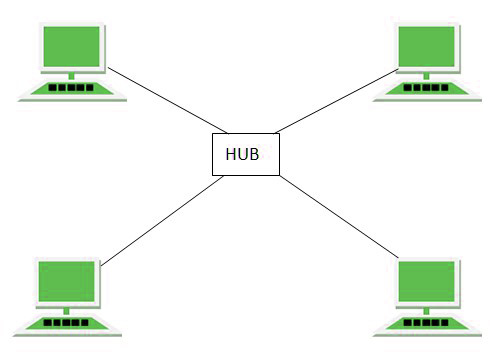
\includegraphics[scale=0.5]{P1/img/Tupen2.jpg}
    \end{center}
	\item Semua perangkat langsung terhubung ke router utama sehingga tidak terdapat sebuah perantara yang mengakibatkan tidak dibutuhkan adanya sebuah gateway dan interface menunjukkan destinasi paket akan dikirimkan untuk masing-masing subnet.
	{\small
		\begin{center}
		\begin{tabular}{ |c|c|c|c| } 
			\hline
			Destinasi Network & Netmask/prefix & Gateway & Interface \\
			\hline
			192.168.0.0 & 255.255.255.128/25 & - & RnD (Gig0/0)  \\
			192.168.0.128 & 255.255.255.192/26 & - & Produksi (Gig0/1)  \\
			192.168.0.192 & 255.255.255.224/27 & - & Administrasi (Gig0/2)  \\
			192.168.0.224 & 255.255.255.240/28 & - & Keuangan (Gig0/3)  \\
			\hline
		\end{tabular}
		\end{center}
	}
	\item Jenis routing yang paling cocok untuk topologi jaringan perusahaan ini adalah static routing yang dikombinasikan dengan teknik Classless Inter-Domain Routing (CIDR). Static routing sangat sesuai karena topologi jaringan berskala kecil dan tetap dan hanya terdiri dari empat subnet yang saling terhubung melalui satu router utama. Konfigurasi static routing sederhana dan tidak membutuhkan overhead protokol dinamis, serta memudahkan administrator dalam mengelola dan memantau lalu lintas jaringan. Penggunaan CIDR memungkinkan pengalokasian IP address yang efisien sesuai kebutuhan tiap departemen, sehingga tidak ada pemborosan alamat IP. CIDR juga memberikan fleksibilitas dalam manajemen subnetting, yang penting dalam perencanaan jangka panjang jaringan internal perusahaan.
\end{enumerate}